% $Header: 
%/cvsroot/latex-beamer/latex-beamer/solutions/conference-talks/conference-ornate-20min.en.tex,v
% 1.6 2004/10/07 20:53:08 tantau Exp $

\documentclass{beamer}

\mode<presentation>
{
%  \usetheme{Hannover}
\usetheme[width=0.7in]{Hannover}
% or ...

  \setbeamercovered{transparent}
  % or whatever (possibly just delete it)
}
\usepackage{longtable}
\usepackage{booktabs}

\usepackage[english]{babel}
% or whatever

\usepackage[latin1]{inputenc}
% or whatever

\usepackage{times}
%\usepackage[T1]{fontenc}
% Or whatever. Note that the encoding and the font should match. If T1
% does not look nice, try deleting the line with the fontenc.
%\usepackage{logictheme}

\usepackage{multirow}
\usepackage{totpages}
\usepackage{hyperref}
\usepackage{booktabs}

\usepackage{listings}
\lstset{columns=flexible}
\usepackage{tikz}
\usetikzlibrary{positioning}

\newcommand{\blt}{- } %used for bullets in a list

\newcounter{datadefnum} %Datadefinition Number
\newcommand{\ddthedatadefnum}{DD\thedatadefnum}
\newcommand{\ddref}[1]{DD\ref{#1}}

\newcommand{\colAwidth}{0.1\textwidth}
\newcommand{\colBwidth}{0.8\textwidth}

\renewcommand{\arraystretch}{1.1} %so that tables with equations do not look 
%crowded

\pgfdeclareimage[height=0.7cm]{logo}{McMasterLogo}
\title[\pgfuseimage{logo}] % (optional, use only with long paper titles)
{GOOL: A Generic Object-Oriented Language}

%\subtitle
%{Include Only If Paper Has a Subtitle}

\author[Slide \thepage~of \pageref{TotPages}] % (optional, use only with lots of
                                              % authors)
{\underline{Jacques Carette}, Brooks MacLachlan, and Spencer Smith}
% - Give the names in the same order as the appear in the paper.
% - Use the \inst{?} command only if the authors have different
%   affiliation.

\institute[McMaster University] % (optional, but mostly needed)
{
  Computing and Software Department\\
  Faculty of Engineering\\
  McMaster University
}
% - Use the \inst command only if there are several affiliations.
% - Keep it simple, no one is interested in your street address.

\date[Jan 20, 2020] % (optional, should be abbreviation of conference name)
{PEPM 2020}
% - Either use conference name or its abbreviation.
% - Not really informative to the audience, more for people (including
%   yourself) who are reading the slides online

%\subject{computational science and engineering, software engineering, software
%  quality, literate programming, software requirements specification, document
%  driven design}
% This is only inserted into the PDF information catalog. Can be left
% out. 

% If you have a file called "university-logo-filename.xxx", where xxx
% is a graphic format that can be processed by latex or pdflatex,
% resp., then you can add a logo as follows:

%\pgfdeclareimage[height=0.5cm]{Mac-logo}{McMasterLogo}
%\logo{\pgfuseimage{Mac-logo}}

% Delete this, if you do not want the table of contents to pop up at
% the beginning of each subsection:
% \AtBeginSubsection[]
% {
%   \begin{frame}<beamer>
%     \frametitle{Outline}
%     \tableofcontents[currentsection,currentsubsection]
%   \end{frame}
% }

% If you wish to uncover everything in a step-wise fashion, uncomment
% the following command: 

%\beamerdefaultoverlayspecification{<+->}

\beamertemplatenavigationsymbolsempty 

\usepackage{color}

\newcommand{\authornote}[3]{\textcolor{#1}{[#3 ---#2]}}
\newcommand{\bmac}[1]{\authornote{red}{BM}{#1}}
\newcommand{\jc}[1]{\authornote{purple}{JC}{#1}}

%% Useful abbreviations
\newcommand{\Csharp}{C\#}
\newcommand{\Cplusplus}{C\texttt{++}}

\begin{document}

%%%%%%%%%%%%%%%%%%%%%%%%%%%%%%%%%%%%%%
\hoffset=-.4in %removing side bar for these frames
\begin{frame}[plain]

\titlepage

\end{frame}
\hoffset=0in %restore

%%%%%%%%%%%%%%%%%%%%%%%%%%%%%%%%%%%%%%

\section[Introduction]{Introduction}

%%%%%%%%%%%%%%%%%%%%%%%%%%%%%%%%%%%%%%

\begin{frame}

\frametitle{Observations}

OO languages:
\begin{itemize}
  \item Structurally similar
  \item Differences are mostly syntactic
  \item Like Romance languages
  \item We tend to say similar things in all of them
\end{itemize}

\end{frame}

%%%%%%%%%%%%%%%%%%%%%%%%%%%%%%%%%%%%%%

\begin{frame}

\frametitle{The Goal}

One language to express them all.

\begin{itemize}
  \item Is it possible?
  \item Capture the meaning of OO programs
  \item DSL for domain of OO programs
  \item GOOL currently targets Java, Python, \Csharp, \Cplusplus
\end{itemize}

\end{frame}

%%%%%%%%%%%%%%%%%%%%%%%%%%%%%%%%%%%%%%

\section[Requirements]{Requirements}

%%%%%%%%%%%%%%%%%%%%%%%%%%%%%%%%%%%%%%

\begin{frame}

\begin{itemize}
  \item \textbf{mainstream}: Generate code in mainstream languages
  \item \textbf{readable}: Generared code is human-readable
  \item \textbf{idiomatic}: Generated code is idiomatic
  \item \textbf{documented}: Generated code is documented
  \item \textbf{patterns}: Express common OO patterns
  \item \textbf{expressivity}: Language succeeds in expressing real OO 
  programs
  \item \textbf{common}: Commonalities abstracted
\end{itemize}

% \bmac{One slide for each?}
% \jc{No. One slide for the requirements.  Might want to unveil each
%  one at a time, with the rhs being a justification instead of expansion.


\end{frame}

%%%%%%%%%%%%%%%%%%%%%%%%%%%%%%%%%%%%%%

\section[Creation]{Creation}

%%%%%%%%%%%%%%%%%%%%%%%%%%%%%%%%%%%%%%

\begin{frame}

\frametitle{Principles}

% This could be split into 2-3 slides
\begin{itemize}
  \item What we can say vs. want to say vs. need to say (ex. Java 
  introspection, \Cplusplus templates)
  \item Readability features i.e. blocks
  \item Variables vs. values
  \item Smart constructors for common idioms
\end{itemize}

\end{frame}

%%%%%%%%%%%%%%%%%%%%%%%%%%%%%%%%%%%%%%

\begin{frame}[fragile] \label{goal}

\frametitle{GOOL Language}

% excellent!
\tiny
\begin{tabular}{p{1.5cm}| p{7cm}}
  Types & \verb|bool|, \verb|int|, \verb|float|, \verb|char|, 
  \verb|string|, 
  \verb|infile| (read mode), \verb|outfile| (write mode), 
  \verb|listType|, 
  \verb|obj| \\
  Variables & \verb|var|, \verb|extVar|, \verb|classVar|, \verb|objVar|, 
  \verb|$->| (infix operator for \verb|objVar|), \verb|self|,
  [\verb|listVar|] \\
  Values & \verb|valueOf| (value from variable), \verb|litTrue|, 
  \verb|litFalse|, \verb|litInt|, 
  \verb|litFloat|, \verb|litChar|, \verb|litString|, \verb|?!|, 
  \verb|?&&|, 
  \verb|?<|, \verb|?<=|, \verb|?>|, \verb|?>=|, \verb|?==|, \verb|?!=|, 
  \verb|#~|, \verb|#/^|, \verb|#||, \verb|#+|, \verb|#-|, \verb|#*|, 
  \verb|#/|, \verb|#^|, \verb|inlineIf|, \verb|funcApp|, 
  \verb|extFuncApp|, 
  \verb|newObj|, \verb|objMethodCall|, [\verb|selfFuncApp|, 
  \verb|objMethodCallNoParams|] \\
  Statements & \verb|varDec|, \verb|varDecDef|, \verb|assign|, \verb|&=|, 
  \verb|&+=|, \verb|&-=|, \verb|&++|, \verb|&~-|, \verb|break|, 
  \verb|continue|, \verb|returnState|, \verb|throw|, \verb|free|, 
  \verb|comment|, \verb|ifCond|, \verb|ifNoElse|, \verb|switch|, 
  \verb|for|, 
  \verb|forRange|, \verb|forEach|, \verb|while|, \verb|tryCatch|, 
  \verb|block|, \verb|body| [\verb|bodyStatements| (single-block body), 
  \verb|oneLiner| (single-statement body)] \\
  List API & \verb|listAccess|, \verb|at| (same as \verb|listAccess|), 
  \verb|listSet|, \verb|listAppend|, \verb|listIndexExists|, 
  \verb|indexOf|, \verb|listSlice| \\
  Scope & \verb|public|, \verb|private| \\
  Binding & \verb|static_|, \verb|dynamic_| \\
  Functions & \verb|function|, \verb|method|, \verb|param|, 
  \verb|pointerParam|, \verb|mainFunction|, \verb|docFunc|, 
  [\verb|pubMethod|, \verb|privMethod|] \\
  State Variables & \verb|stateVar|, \verb|constVar|, [\verb|privMVar|, 
  \verb|pubMVar| (dynamic), \verb|pubGVar| (static)]\\
  Classes & \verb|buildClass|, \verb|docClass|, [\verb|pubClass|, 
  \verb|privClass|]\\
  Packages & \verb|buildModule|, \verb|fileDoc|, \verb|docMod|, 
  \verb|prog|, 
  \verb|package|, \verb|doxConfig|, \verb|makefile|
\end{tabular}

\end{frame}

%%%%%%%%%%%%%%%%%%%%%%%%%%%%%%%%%%%%%%

\section[Implementation]{Implementation}

%%%%%%%%%%%%%%%%%%%%%%%%%%%%%%%%%%%%%%

\begin{frame}[fragile]

\frametitle{Encoding}

Tagless with type families -- 2 Layers of abstraction
\begin{itemize}
  \item Over target language
  \item Over underlying data structures
\end{itemize}

% make sure to load the language 'haskell' here.
\begin{lstlisting}
class (TypeSym repr) => VariableSym repr where
  type Variable repr
  var :: Label -> repr (Type repr)
    -> repr (Variable repr)
\end{lstlisting}

\end{frame}

%%%%%%%%%%%%%%%%%%%%%%%%%%%%%%%%%%%%%%

\begin{frame}
\centering
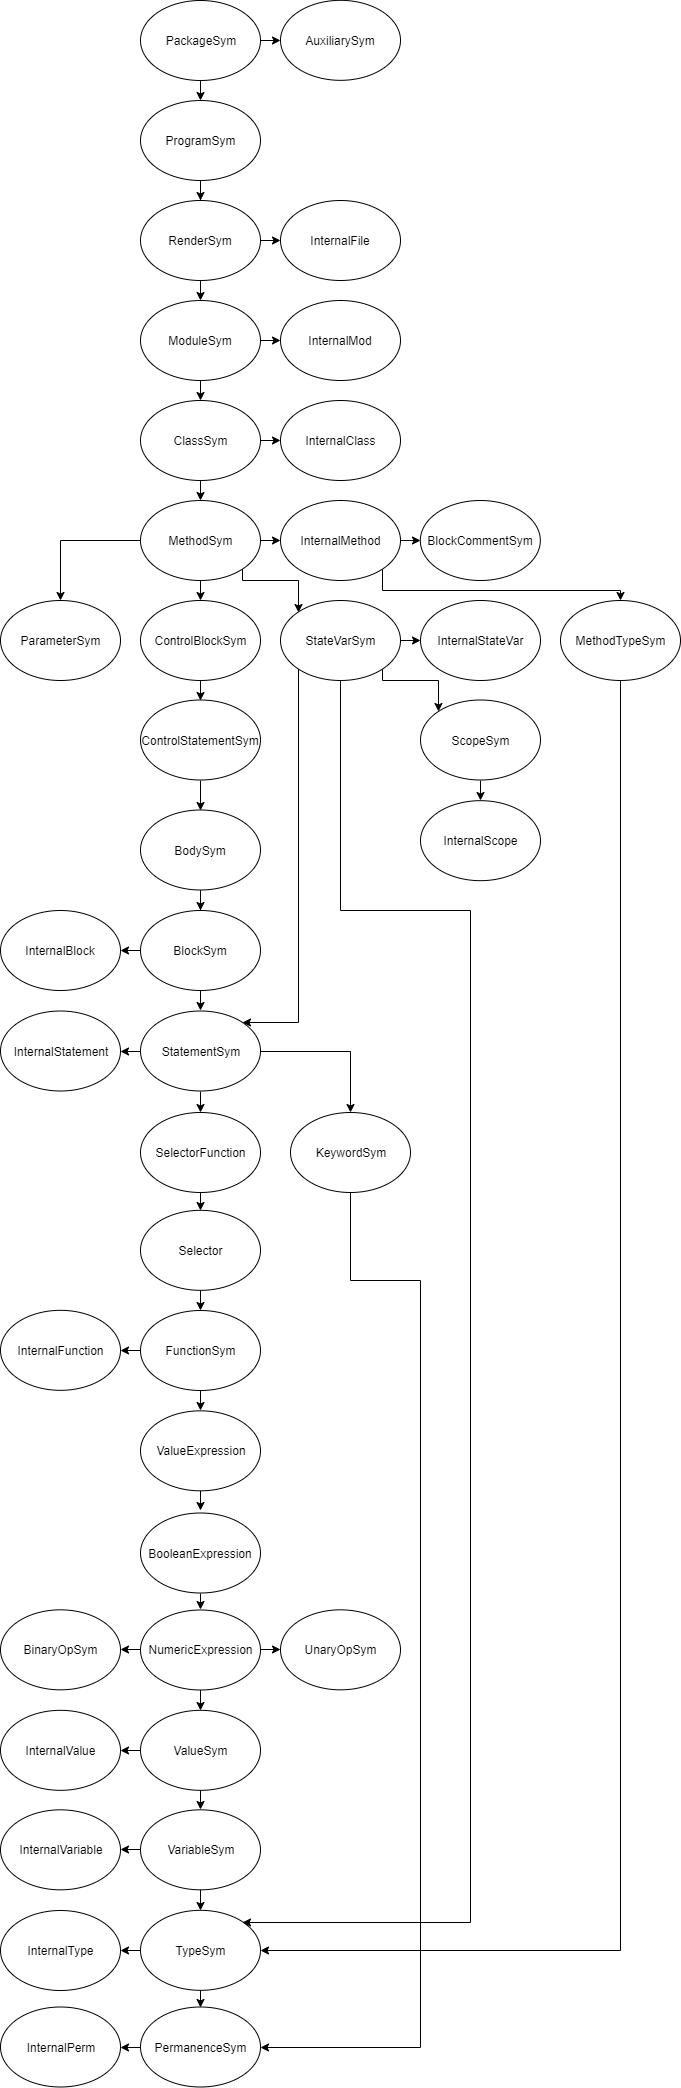
\includegraphics[scale=0.12]{GOOLClasses.png}

% \bmac{Very squished to fit in frame, should we keep this?}
% \jc{Yes - but also have a side-by side version of the top half / bottom
% half that is more readable}
\end{frame}

%%%%%%%%%%%%%%%%%%%%%%%%%%%%%%%%%%%%%%

\begin{frame}

\frametitle{Statistics}

\begin{itemize}
  \item 43 classes
  \item 328 methods
  \item 300 functions that abstract over commonalities
  \item 229 methods shared between Java and \Csharp
  \begin{itemize}
      \item 40\% more than between Java and Python
  \end{itemize}
\end{itemize}

\bmac{Include the bar graph of common methods from long version of paper?}
	\jc{yes please}

\end{frame}

%%%%%%%%%%%%%%%%%%%%%%%%%%%%%%%%%%%%%%

\section[Patterns]{Patterns}

%%%%%%%%%%%%%%%%%%%%%%%%%%%%%%%%%%%%%%

\begin{frame}

\frametitle{Patterns}

\begin{itemize}
  \item Command line arguments
  \item Lists
  \item I/O
  \item Procedures with Input/Output/Both parameters
  \item Getters and setters
  \item Design patterns
\end{itemize}

%\bmac{Do we want to mention all of these? A slide with sample code for each? Or 
%maybe pick one to use as an example? GOOL code, generated code, or both?}
% \jc{Pick maybe 2 as examples, with all artifacts?}
\end{frame}

%%%%%%%%%%%%%%%%%%%%%%%%%%%%%%%%%%%%%%

\begin{frame}

\frametitle{Demo?}

\jc{Short papers \emph{may} include a demo, but don't have to.}
\bmac{Maybe show the PatternTest example like we do in the long version of the 
paper. Can show GOOL code and target code in all languages. Would probably want 
to leave the slideshow for this demo?}

\bmac{I can alternatively write up a new ``test'' for the purpose of this demo, 
if you want to request some specific features to show off or if you have a 
specific idea}

\end{frame}

%%%%%%%%%%%%%%%%%%%%%%%%%%%%%%%%%%%%%%

\section[Conclusions]{Conclusions}

%%%%%%%%%%%%%%%%%%%%%%%%%%%%%%%%%%%%%%

\begin{frame}

\frametitle{Future}

\begin{itemize}
  \item More types
  \item Smarter generation using State monad - ex. import statements
  \item Interface with external libraries
  \item User-decisions - ex. which type to use for lists?
  \item More patterns
\end{itemize}

\bmac{Split into a slide for each? Or pick a couple important ones and just do 
a slide for each of those?}

\end{frame}

%%%%%%%%%%%%%%%%%%%%%%%%%%%%%%%%%%%%%%

\begin{frame}

\frametitle{Conclusion}

We currently use GOOL to generate some examples of scientific software (glass 
breakage, projectile simulation)\\~\

Together new:
\begin{itemize}
  \item Idiomatic code generation
  \item Human-readable, documented code generation
  \item Coding patterns are language idioms\\~\
\end{itemize}

With respect to ``\hyperref[goal]{The Goal}'' --- It is possible\\~\

% \bmac{We don't need to discuss related work in the presentation, do we?}
% \jc{no}

\end{frame}

\end{document}
